\begin{figure}[htb]
  \centering
  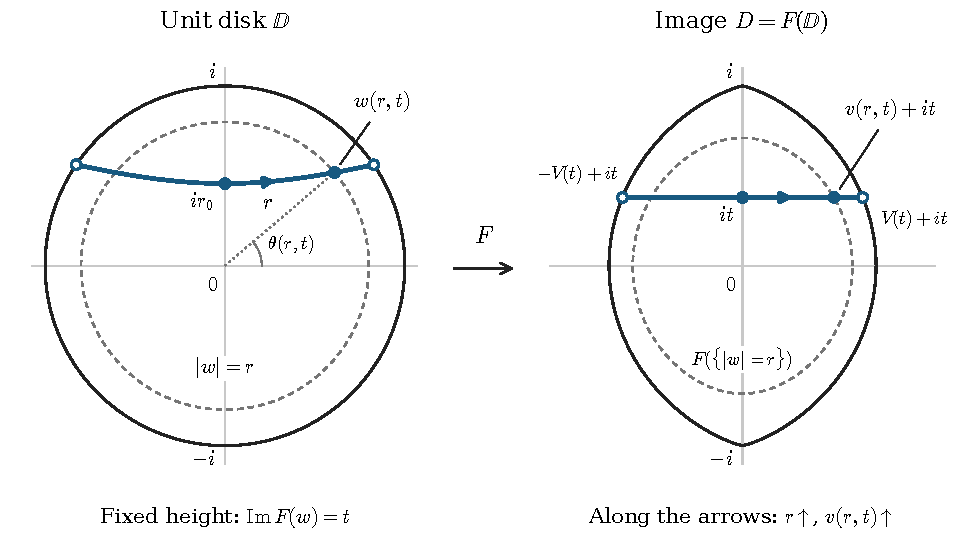
\includegraphics[width=\linewidth]{figures/lens-slices.pdf}
  \caption{A fixed horizontal slice and its preimage, illustrated for $t>0$.
  Along the right half of the highlighted preimage curve in the left panel,
  $r$ increases from
  $r_0=T^{-1}(t)$ to $1$, while $v(r,t)$ increases from $0$ to $V(t)$.
  The dashed circle and its image pass through the corresponding marked
  points. Open markers indicate boundary limits.}
  \label{fig:lens-slices}
\end{figure}
